\subsection*{Dataset} \label{sec:dataset}
The dataset consists of 105 aneurysm 3D meshes, created by intersecting an ideal half torus with aneurysm bulges extracted from patient cases in the \textit{IntrA} dataset \cite{yang_intra_2020}, following Goetz et al. methodology \cite{goetz_anxplore_2024}. \firstround We refer to them as semi-idealized geometries, as they combine an idealized toroidal parent artery with a patient-specific aneurysm bulge, as illustrated in \autoref{fig:anxplore}.

These chosen geometries represent sidewall aneurysms located on the internal carotid artery (ICA), particularly near the ICA siphon. This choice is motivated by its clinical representativeness: the ICA siphon region is a common site for aneurysm formation and is frequently modeled in hemodynamic studies due to its characteristic curvature \citep{ramalho_influence_2013}. Several prior works have highlighted the ICA’s susceptibility to aneurysm development at curved segments due to altered flow patterns and wall shear stress concentrations \cite{sunderland_disturbed_2022}. Notably, the siphon’s curvature is often approximated as toroidal, making the torus-shaped backbone both anatomically justified and reproducible across computational settings. \color{black}

\begin{figure}[!ht]
    \centering
    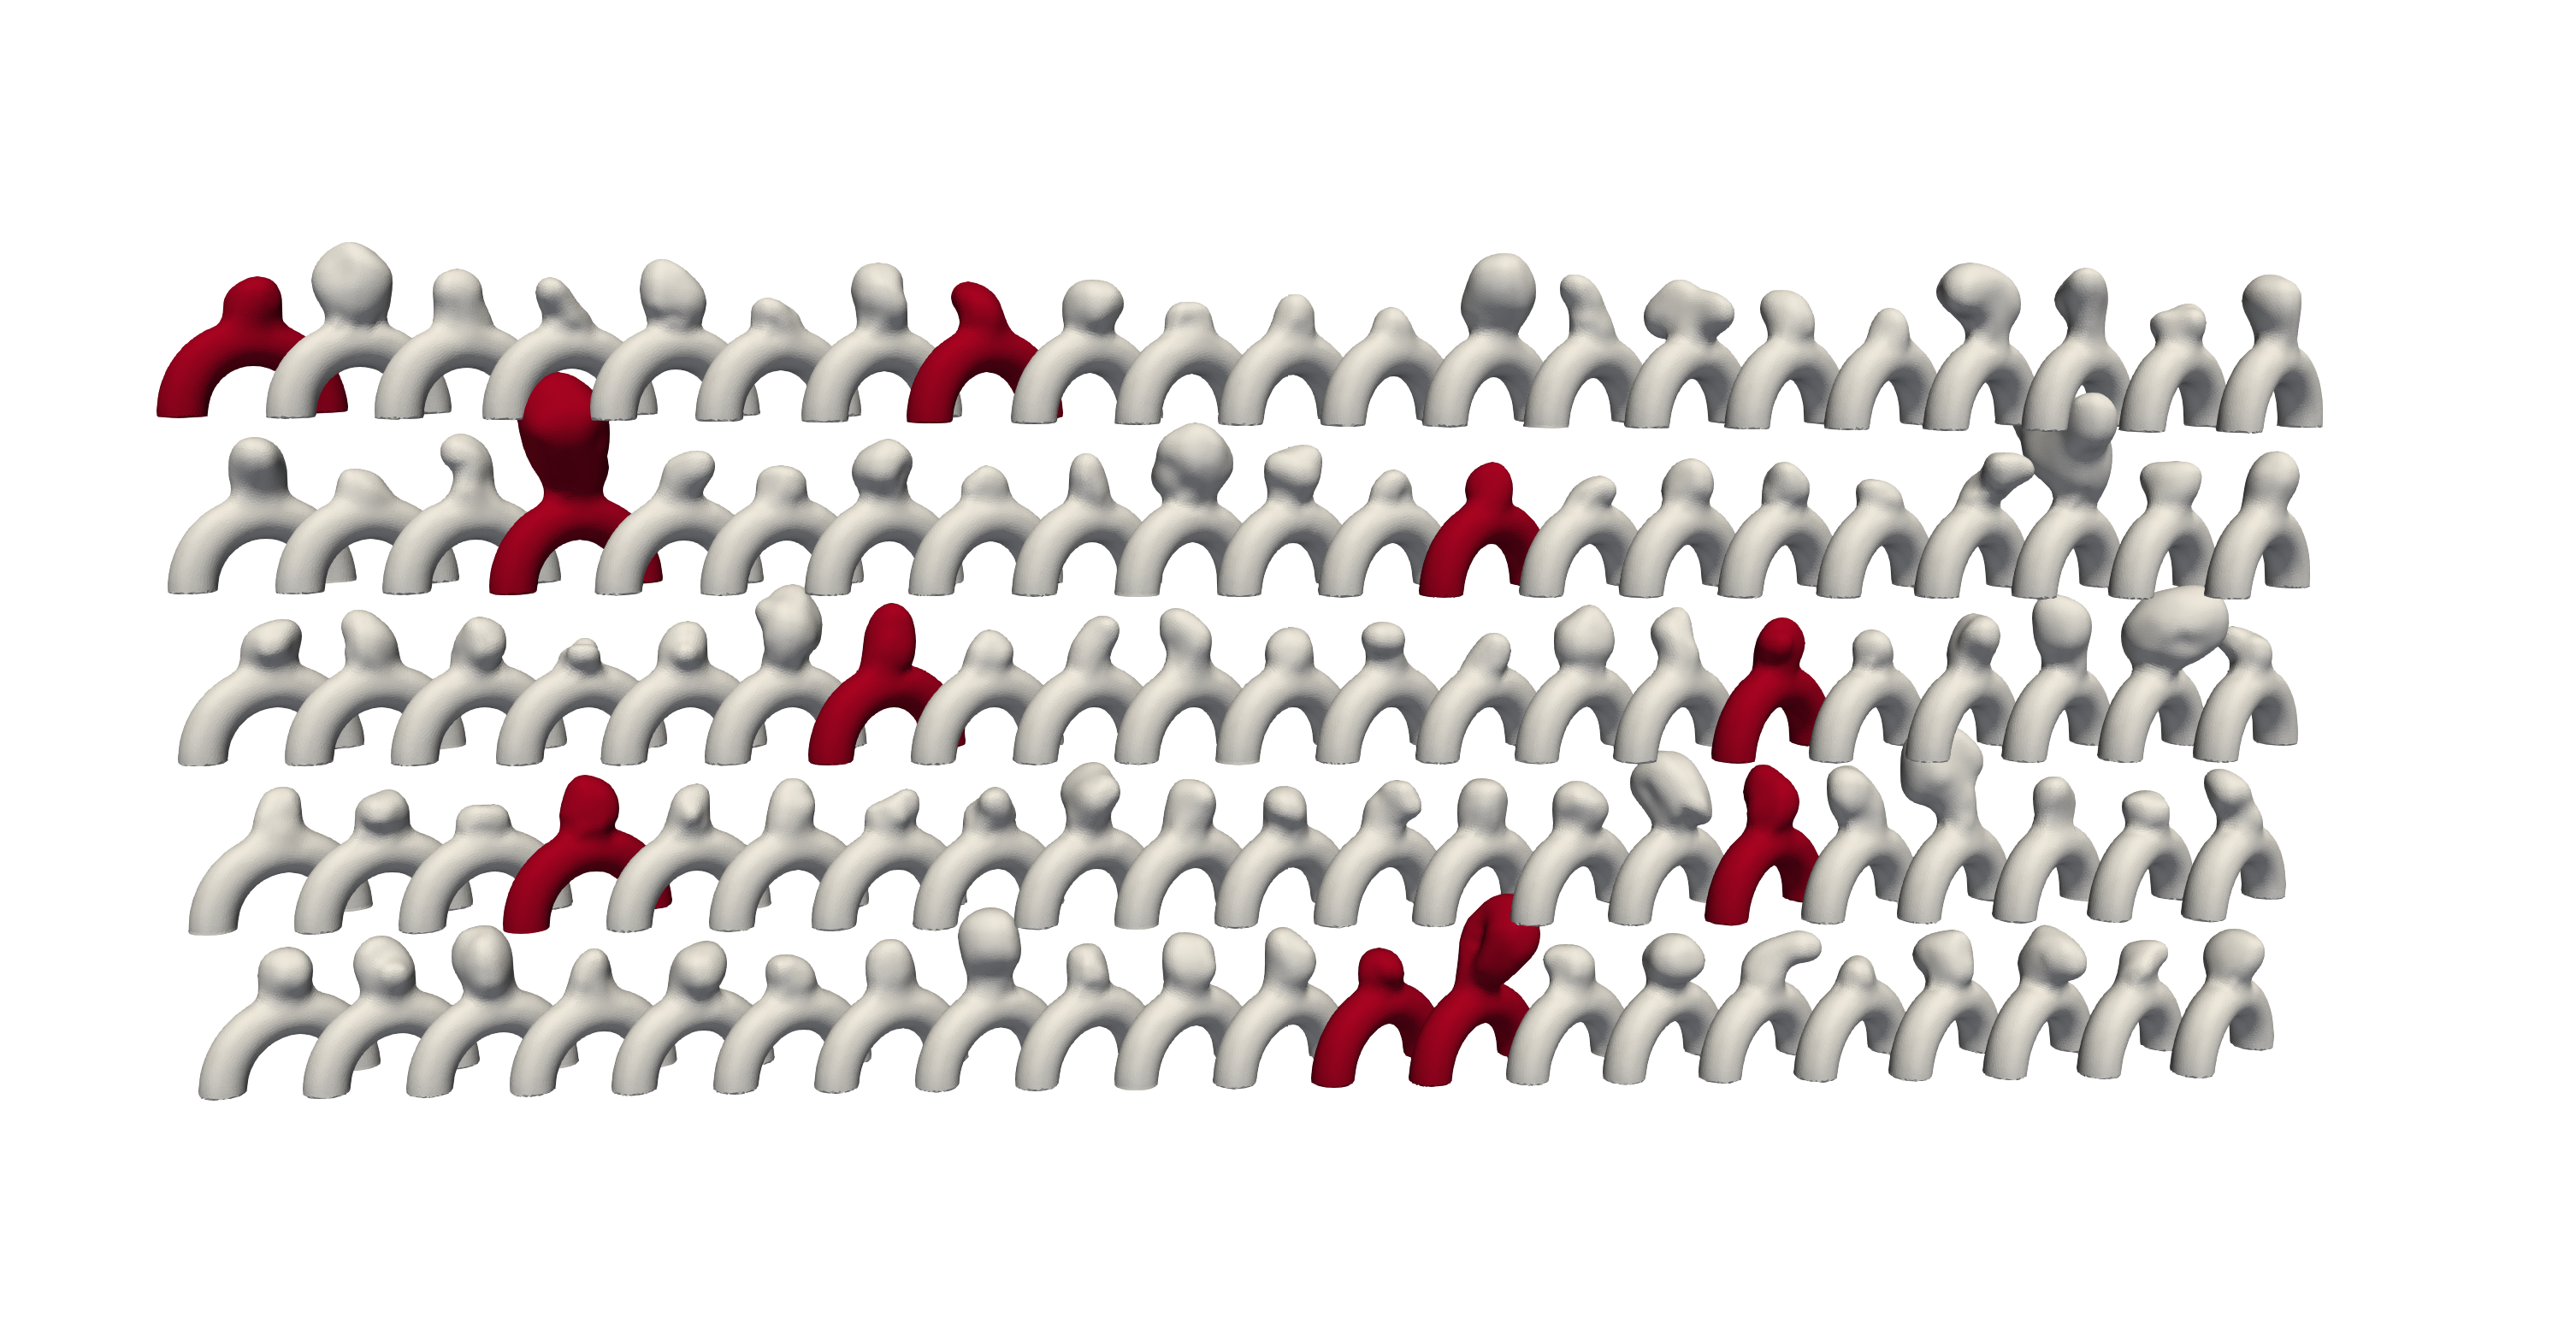
\includegraphics[width=1\textwidth, trim={150 250 250 250}, clip]{figs/anxplore_dataset.png.png}
    \caption{Dataset of 105 semi-idealised patient-specific geometries \cite{goetz_anxplore_2024} with 10 highlighted test cases.}
    \label{fig:anxplore}
\end{figure}

\firstround The bulges range from 3 to 9 mm in diameter, covering diverse pathological shapes and the selected vessel diameter in our dataset is 4 mm, which aligns with clinical measurements of the ICA in adult patients typically ranging from 3–6 mm \cite{baz_morphometry_2021}. 

\thirdround We generated the \textbf{BenchAnXplore} dataset following the meshing, coarsening and simulation processes further detailed in the \nameref{sec:Methods} section, and obtained 105 aneurysm geometries, with 80 simulated timeframes for each of these cases. This dataset is now made available as a benchmark case for AI intracranial aneurysms applications. \color{black}


\subsection*{Training} \label{sec:training}
We trained and compared four models to evaluate the impact of node feature enhancement and physically-informed improvements separately. To ensure a fair comparison, all models were trained using the same configuration. \firstround All MLPs (multilayer perceptrons) used for encoders, decoders and update functions within the GN blocks, have two hidden layers of 128 neurons each, \secondround and use a ReLU activation function. \color{black} We used 15 rounds of message passing, bringing the total number of parameters to approximately 3 million.

With 105 simulations, each spanning 80 timesteps, we trained on 95 simulations and randomly selected 10 for testing and evaluation (highlighted in red in \autoref{fig:anxplore}). This test set gathers a wide variety in shapes and flow characteristics as depicted in \autoref{fig:test_set}. Given that our meshes contain in average 20,000 nodes, this results in over 75 million training tokens. Recall that number of training tokens is equal to trajectories * timesteps * data points.

%  Our model having approximately 290k trainable parameters, the number 
We trained for 20 epochs e.g. 144k training steps, using a fixed learning rate \secondround of $10^{-4}$ \color{black} for 16 epochs followed by 4 epochs with exponential decay \secondround to reach a minimum learning rate of $10^{-7}$. \color{black}Training was conducted on L4 NVIDIA GPUs, taking approximately 20 hours, with a slight ($\sim 5$\%) increase for the physically informed network due to gradient computations.

% flops calculation :
% nb of training tokens = 80t * 91traj * 10k nodes = 72.8 millions
% flops = training tokens * 290k params = 2.1e13

\begin{figure}[!ht]
    \centering
    \includegraphics[width=0.70\textwidth, trim={620 0 700 50}, clip]{figs/testset.png}
    \caption{Test set of 10 representative blood flow CFD simulations.}
    \label{fig:test_set}
\end{figure}

\paragraph{Boundary conditions} To handle boundary conditions over the domain, we added a node type as an input feature to separate different training behaviors according to the considered nodes. We fixed a null velocity for the wall nodes and did not compute loss nor performed learning onto these nodes. The velocity at the inlet nodes was fixed; we imposed the same pulsatile parabolic inflow profile as in the ground-truth CFD simulations. All other nodes of the fluid domain, outflow included, were used to train the network.

\paragraph{Training noise} Our models are trained for 1-step prediction tasks but are intended to be used in a "rollout" scenario, where they iteratively use their own predictions to generate an entire simulation. In such scenarios, the model's input data can deviate from the training distribution due to errors introduced in previous steps. This deviation amplifies errors over successive iterations, resulting in cumulative inaccuracies throughout the simulation. Following the same strategy as \cite{sanchez-gonzalez_learning_2020}, we introduced noise to all our dynamical variables during training to enhance the robustness of our models. 

\paragraph{Timestep} To simplify training and eliminate temporal ambiguity, we fixed the training timestep to 0.01 s, which is coarser than the CFD solver’s timestep of 0.001 s. This was done intentionally to reduce sequence length while maintaining temporal coherence. As such, the model is not required to generalize to arbitrary time horizons. While we did not test interpolation across multiple timestep sizes, the current design is adequate for clinical use cases where a consistent frame rate is expected. \color{black}

\begin{figure}[!ht]
    \centering
    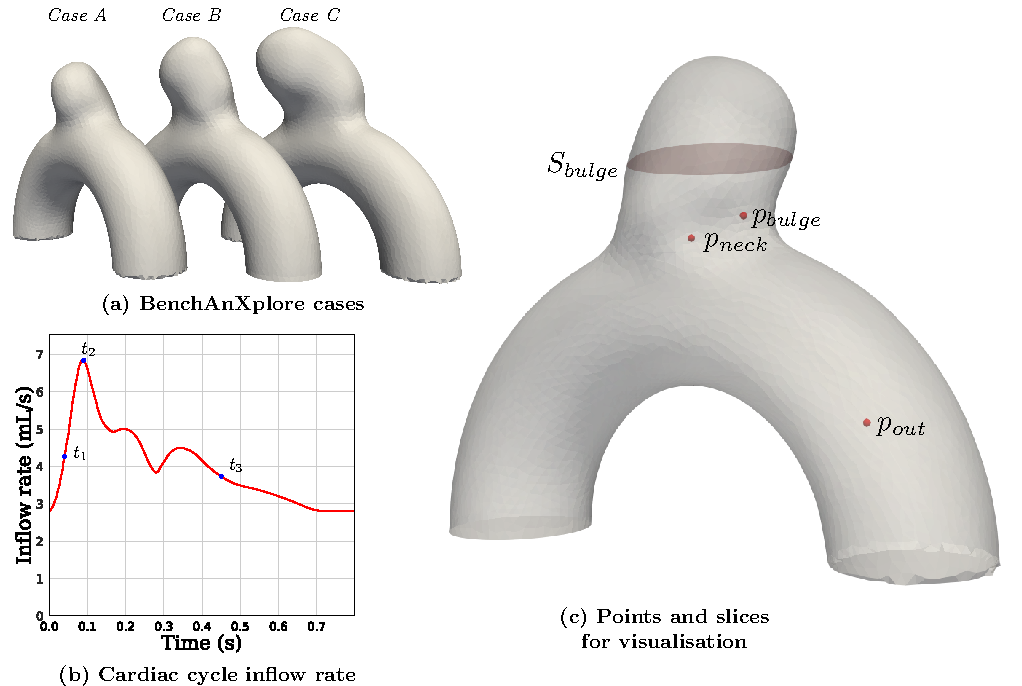
\includegraphics[width=0.9\textwidth]{figs/evalutation_cases.pdf}
    \caption{Evaluation cases with \textbf{(a)}: cases chosen from our testing dataset for deeper analysis; \textbf{(b)}: pulsatile inflow rate, with 3 chosen time frames for evaluation; \textbf{(c)}: slice and points used for velocity data extraction.}
    \label{fig:eval_cases}
\end{figure}

\subsection*{Numerical performance}

We evaluated all four models on the full test set for both next-step and rollout prediction with 1-step and 50-step Root Mean Square Errors (RMSE) as described in the \nameref{sec:Methods} section; mean errors over all test cases are given in \autoref{tab:model-configurations}. While all models perform well on next-step prediction, as shown by the 1-step error in \autoref{tab:model-configurations}, significant differences emerge in rollout prediction in particular at time $t_2$ as clearly highlighted in  \autoref{fig:model_comparison}. 

\begin{figure}[!ht]
    \centering
    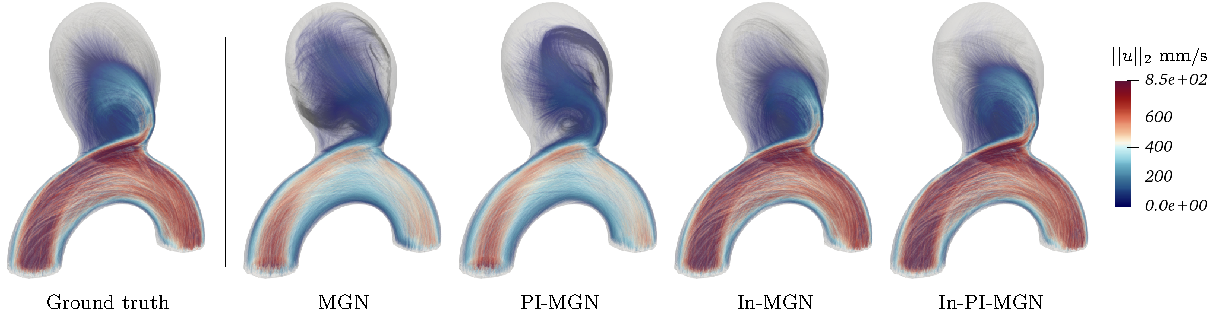
\includegraphics[width=1.05\textwidth]{figs/model_rollout_comp.pdf}
\caption{Rollout predictions at time $t_2$ for all trained models.}
\label{fig:model_comparison}
\end{figure}

Indeed, the In-MGN and In-PI-MGN models produce high-quality rollouts, with the 50-step error for In-PI-MGN being more than six times lower than the MGN baseline. In-MGN also performs well on longer predictions, whereas introducing the physical loss alone does not improve long-term prediction performance. Both MGN and PI-MGN models converge for single-step predictions but struggle with error accumulation in rollout predictions. 

\begin{table}[ht]
    \centering
    \begin{tabular}{l c c c c c}
        \toprule
        \textbf{Model} & \textbf{Input features} & \textbf{Loss function} & \textbf{1-RMSE} & \textbf{50-RMSE} & \firstround \textbf{50-RMSE SD}\color{black}\\
        \midrule \midrule
        \text{MGN} & $u$ & $\mathcal{L}_{data}$ & 1.11 & 50.51 & \firstround 1.43\color{black}\\
        \text{PI-MGN} & $u$ & $\mathcal{L}_{PI}$ & \textit{1.06} & 55.62 & \firstround 1.27\color{black}\\
        \text{In-MGN} & $u$, $du/dt$, inflow & $\mathcal{L}_{data}$ & 1.09 & \textit{9.22} & \firstround 1.47\color{black}\\
        \text{In-PI-MGN} & $u$, $du/dt$, inflow & $\mathcal{L}_{PI}$ & \textbf{0.85} & \textbf{7.58} & \firstround 1.02\color{black}\\
        \bottomrule
    \end{tabular}
    \caption{Model configurations and performance. \firstround Errors averaged on the test set over the whole geometry; next step prediction (1-RMSE) and rollout predictions (50-RMSE) errors are given in mm/s. The standard deviation (SD) of the 50-RMSE across the test set cases is also displayed. Best results are displayed in \textbf{bold}; second best in \textit{italic}}
    \label{tab:model-configurations}
\end{table}


\begin{figure}[!ht]
    \firstround
    \centering
     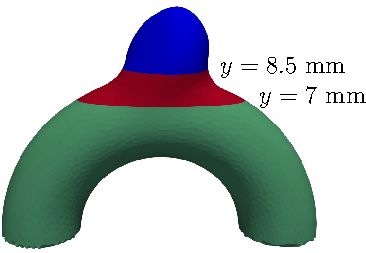
\includegraphics[width=0.3\textwidth]{figs/geometry_zones.pdf}
    \caption{Split of our geometries at planes $y=8.5$ mm and $y=7$ mm to evaluate RMSE metrics in three anatomically regions: the aneurysm bulge (blue), the neck (red) and the parent artery (green).}
    \label{fig:anev_regions}
\end{figure}

\firstround Because all geometries share the same parent artery, averaging the errors over the entire domain may obscure localized variations in model performance. To better assess the predictive accuracy of each model, we computed the 1-step and 50-step RMSEs separately across three anatomically distinct regions: the aneurysm bulge, the neck, and the distal segment of the parent artery (see \autoref{fig:anev_regions}). The results for all four models are summarized in \autoref{tab:results_region}, confirming the same overall tendencies observed in the global error metrics. \color{black}

% \begin{figure}[!ht]
%     \centering
%     \includegraphics[width=0.5\textwidth]{figures/aneurysm_regions.pdf}
% \caption{Split of our geometries at planes $y = 8.5$ and $y=7$ to evaluate RMSE metrics in three regions: the aneurysm bulge (blue), the neck (red) and the parent artery (green).}
% \label{fig:model_comparison}
% \end{figure}

\begin{table}[ht]
    \firstround
    \centering
    \begin{tabular}{l c c c}
        \toprule
        \textbf{Model} & \textbf{Bulge 1-RMSE} & \textbf{Neck 1-RMSE} & \textbf{Artery 1-RMSE}\\
        \midrule \midrule
        \text{MGN} & 1.22 & 1.63 & 0.91 \\
        \text{PI-MGN} & 1.14 & \textit{1.31} & 0.92 \\
        \text{In-MGN} & \textit{1.11} & 1.47 & \textit{0.83} \\
        \text{In-PI-MGN} & \textbf{0.68} & \textbf{1.16} & \textbf{0.74} \\
        
        \midrule
        \textbf{Model} & \textbf{Bulge 50-RMSE} & \textbf{Neck 50-RMSE} & \textbf{Artery 50-RMSE}\\
        \midrule \midrule
        \text{MGN} & 38.16 & 62.25 & 51.77 \\
        \text{PI-MGN} & 44.88 & 66.01 & 57.87 \\
        \text{In-MGN} & \textit{18.28} & \textit{10.66} & \textbf{4.62} \\
        \text{In-PI-MGN} & \textbf{11.87} & \textbf{8.38} & \textit{4.66} \\
        \bottomrule
    \end{tabular}
    \caption{1-RMSE and 50-RMSE in mm/s averaged across the test set on the different regions of the geometries. Best results are displayed in \textbf{bold}; second best in \textit{italic}.}
    \label{tab:results_region}
\end{table}

\firstround To assess the individual impact of acceleration and inflow information on model performance, we conducted an ablation study as part of our experiments. The results showed that adding inflow features alone improved both training convergence and long-term rollout predictions, whereas adding acceleration without inflow features did not lead to model convergence. This suggests that local temporal history is insufficient for accurate prediction in the absence of global context. The combination of both inflow and acceleration features yielded the best performance in terms of error metrics and qualitative agreement with CFD fields. \color{black}



Figures \ref{fig:streamlines_time} and \ref{fig:streamlines_case_c} show a temporal analysis of the full geometry volume. It clearly demonstrate that GNN predictions are closely aligned with ground truth CFD simulations, even during the systolic phase, where velocity fluctuations are pronounced. Additionally, the model effectively captures the evolution of recirculation within the aneurysm bulge. To assess the model’s performance across a diverse range of flow characteristics and bulge shapes, velocity predictions were generated for the entire test set, as illustrated in \autoref{fig:test_comparison}. 

\begin{figure}[!ht]
    \centering
    \includegraphics[width=0.98\textwidth]{figs/timeflow_B.pdf}
    \caption{Blood flow during systole for Case B, showing predictions closely matching simulations throughout the acceleration phase}
    \label{fig:streamlines_time}
\end{figure}

Quantitative comparisons at the aneurysm neck (\autoref{fig:slice_1}) demonstrate good agreement in predicted flow dynamics, particularly where high-velocity jets interact with the aneurysm wall. Velocity measurements at evaluation points (\autoref{fig:point_velocity_comparison}) further illustrate model accuracy. While the baseline MGN model deviates significantly from the ground truth after a few timesteps, both inflow enhanced In-MGN and In-PI-MGN maintain an error margin within 5\% for most of the cardiac cycle at $p_{neck}$ and $p_{out}$. Predictions at $p_{wall}$ are less precise for In-MGN and exhibit some delay, whereas In-PI-MGN remains closely aligned with the ground truth, particularly after systole.

\begin{figure}[!ht]
    \centering
    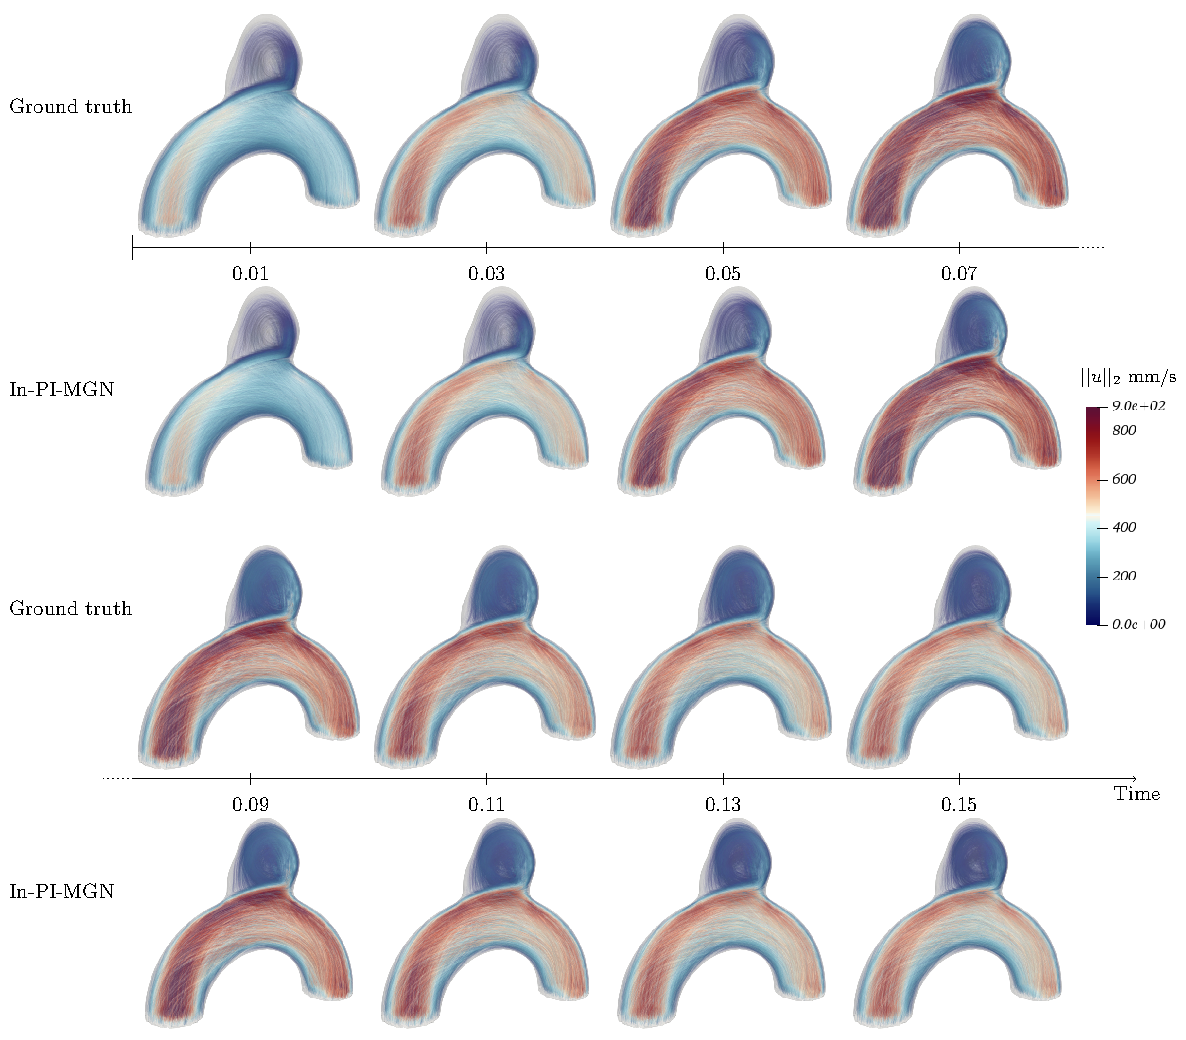
\includegraphics[width=0.98\textwidth]{figs/timeflow_C.pdf}
    \caption{Blood flow during systole for Case C, demonstrating accurate predictions in a larger, more asymmetrical aneurysm bulge.}
    \label{fig:streamlines_case_c}
\end{figure}

\begin{figure}[!ht]
\centering
\includegraphics[width=1\textwidth]{figs/testset_comp.pdf}
\caption{Velocity fields comparison for the whole test set at time $t_2$.}
\label{fig:test_comparison}
\end{figure}

Beyond velocity evaluation, WSS results derived from velocity fields were also analyzed by comparing TAWSS in the aneurysm bulge for the In-PI-MGN model and the ground truth, as shown in \autoref{fig:tawss} and \autoref{fig:time_wss}. The prediction error remains within 10\% across the entire test set, demonstrating strong agreement between predicted and reference patterns. Finally, instant WSS and space-averaged WSS (SAWSS) were examined in \autoref{fig:sawss} to track WSS variations throughout the cardiac cycle. The SAWSS curves indicate that while the In-MGN model follows the general trend, the In-PI-MGN model exhibits the closest match to the reference, particularly in capturing peak values and transient dynamics. The WSS plots at our three evaluation timesteps confirm again the accuracy of the model pattern prediction over the cardiac cycle.

\firstround Furthermore, in order to evaluate the ability of the model to conserve mass, we conducted quantitative mass flow analyses at multiple cross-sectional planes along the artery, as displayed in \autoref{fig:massflow}. Specifically, we measured the instantaneous volumetric flow rates at the inlet, the outlet, and at two additional intermediate planes normal to the centerline of the parent artery. These measurements were performed across the full cardiac cycle for both the CFD ground truth and the In-PI-MGN model predictions.

The results are presented in \autoref{fig:massflow} illustrating the flow rates across the geometry for both the ground truth and the predicted velocity fields. The mean difference between inlet and outlet flow rates for ground truth and prediction are 2.3\% and 3.7\% respectively, with maximums across the cardiac cycle at 2.9\% and 5.2\%. These results further support that the model captures not only the spatial and temporal dynamics of blood flow but also also respects core physical laws such as continuity. \color{black}

\begin{figure}[!ht]
    \centering
    \includegraphics[width=1\textwidth]{figs/neck_slice_comp.pdf}
    \caption{Blood velocity comparison at the aneurysm neck; displayed error is normalized by maximum ground-truth velocity at the given timestep. Maximum error is occurring at high speed flow regions close to the wall, and remains below 8\%.}
    \label{fig:slice_1}
\end{figure}

\begin{figure}[H]
    \centering
    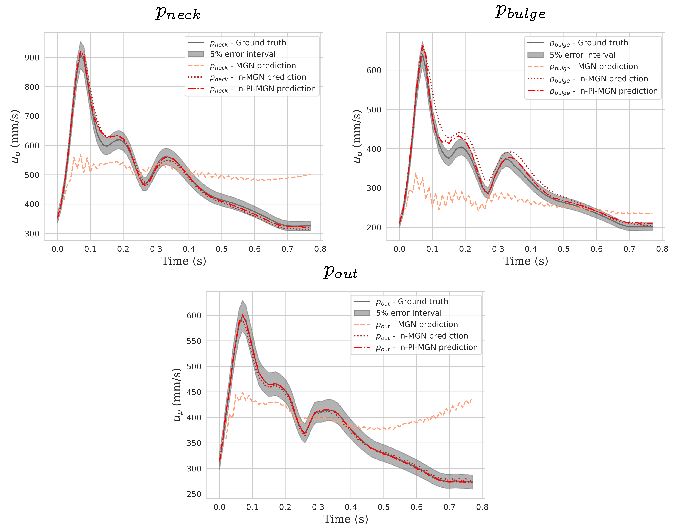
\includegraphics[width=1\textwidth]{figs/point_velocity.pdf.pdf}
\caption{Velocity evolution plotted over time for Case A.}
\label{fig:point_velocity_comparison}
\end{figure}

\begin{figure}[H]
    \centering
    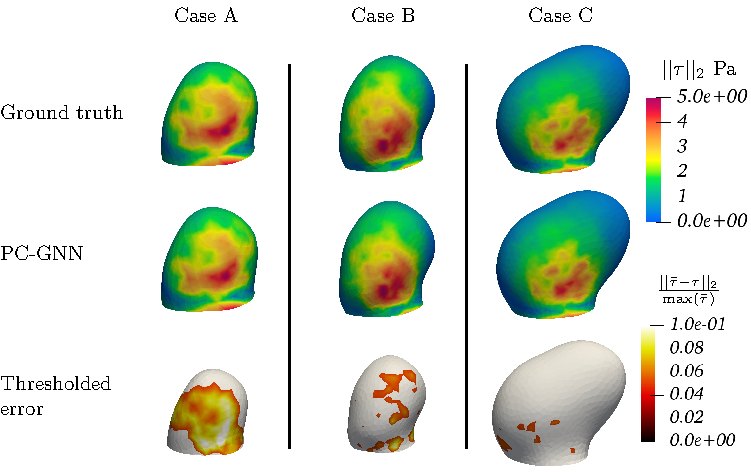
\includegraphics[width=0.7\textwidth]{figs/TAWSS_bulge_comp.pdf.pdf}
    \caption{TAWSS magnitude plotted on the aneurysm bulge, and relative error normalized by maximum ground-truth TAWSS. Error is thresholded to mask errors under 5\%; maximum local error is at 9\%.}
    \label{fig:tawss}
\end{figure}


\begin{figure}[H]
    \centering
    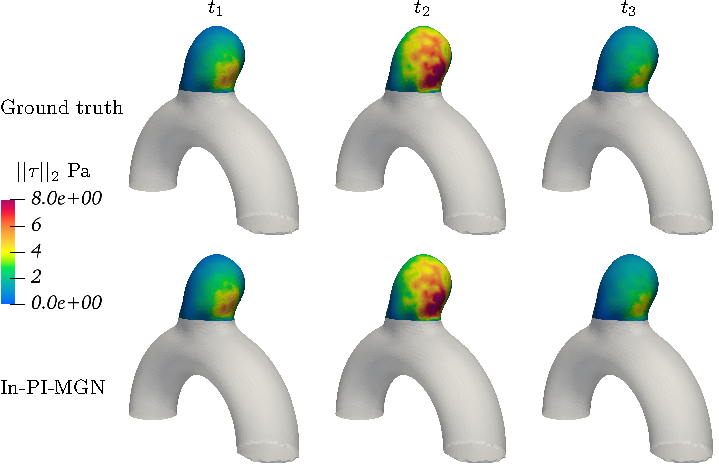
\includegraphics[width=0.7\textwidth]{figs/WSS_bulge_comp.pdf}
    \caption{WSS plotted over the aneurysm bulge at different timeframes for Case B.}
    \label{fig:time_wss}
\end{figure}

\begin{figure}[H]
\centering
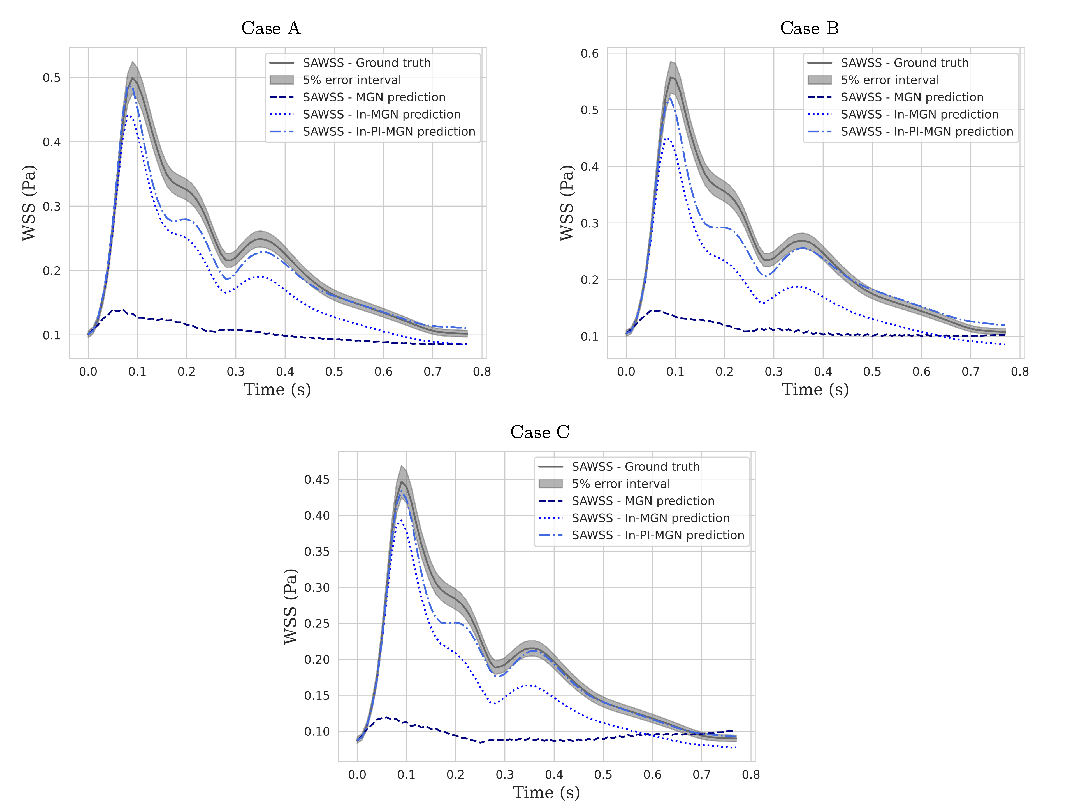
\includegraphics[width=1.1\textwidth]{figs/SAWSS_comp.pdf}
\caption{SAWSS computed over the aneurysm bulge for all 3 test cases.}
\label{fig:sawss}
\end{figure}


\begin{figure}[H]
\firstround
\centering
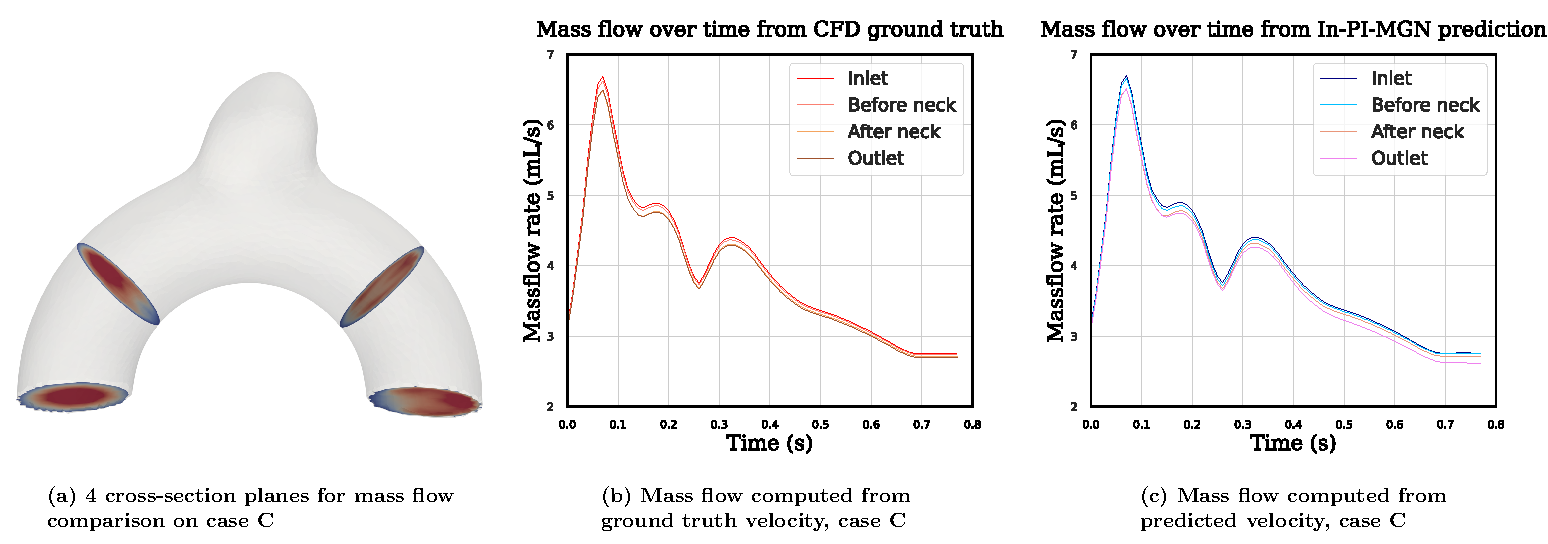
\includegraphics[width=1.1\textwidth]{figs/massflow_comp.pdf}
\caption{Comparison of mass flow on different cross-sections of evaluation case C.}
\label{fig:massflow}
\end{figure}

\secondround 
\subsection*{Generalization to unseen cases}
\color{black}

In order to evaluate the generalization capability of the model trained solely on semi-idealized geometries, we conducted two experiments without any additional fine-tuning. Indeed, the proposed GNN framework operates entirely on local mesh and flow features rather than relying on global geometry descriptors, therefore, it is essential to assess its ability to adapt to new settings, provided the underlying physics and boundary conditions remain comparable.

First, we examined the model’s robustness to unseen inflow rates. We ran new CFD simulations on our three test cases using alternative inflow velocity time profiles from ICA and middle cerebral artery (MCA) as well, derived from the literature \cite{Hoi2011, Reymond2009}, shown in \autoref{fig:inflow_profiles}. When evaluated on these six new inflow conditions (with no retraining), the model achieved a 1-step RMSE of 2.4 and a 50-step RMSE of 14.3. Velocity field comparisons in \autoref{fig:slices_inflow} confirm that predictions remain close to the ground truth, despite never encountering these inflow profiles during training. This result demonstrates the model’s adaptability to physiologically realistic variations in inflow dynamics, even though it was trained on a single fixed profile.

\begin{figure}[!ht]
\firstround
\centering
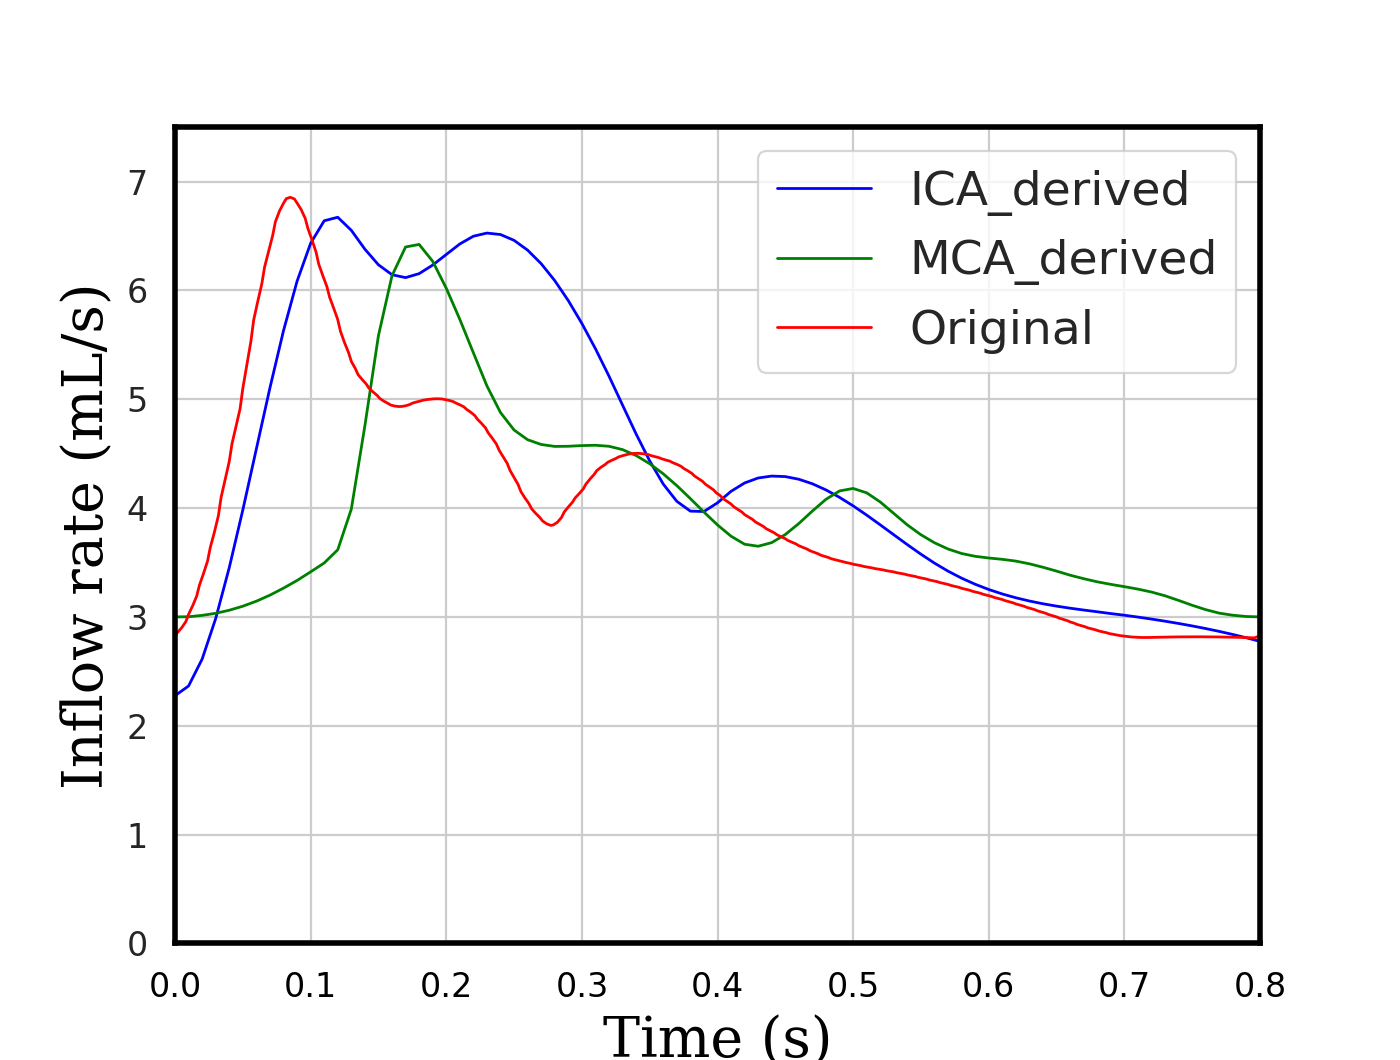
\includegraphics[width=0.6\textwidth]{figs/inflow_rates.png}
\caption{Different inflow rates derived from patient-specific ICA and MCA data \cite{Hoi2011, Reymond2009}.}
\label{fig:inflow_profiles}
\end{figure}

\begin{figure}[!ht]
\firstround
\centering
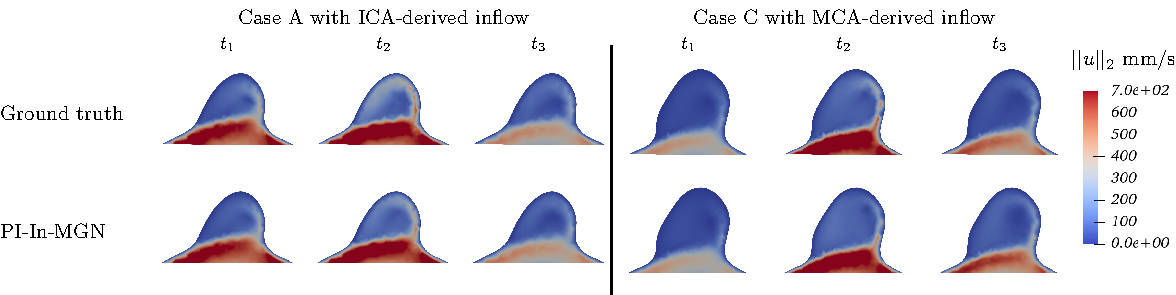
\includegraphics[width=1\textwidth]{figs/neck_velocity_comp.pdf.pdf}
\caption{Blood velocity comparison at the aneurysm neck on unseen velocity profiles.}
\label{fig:slices_inflow}
\end{figure}

\secondround 

Second, we tested the model on four zero-shot predictions on out-of-distribution, patient-specific aneurysm geometries. These new cases were randomly selected from our internal database and exhibit a range of morphological variations, including aneurysm location, parent vessel diameter, neck size, aneurysm sac diameter, and centerline length. Their geometrical features are further described in \autoref{tab:0-shot_cases} and highlight the difference of these cases from the BenchAnXplore training and testing data.

Remarkably, the In-PI-MGN model trained only on synthetic semi-idealized geometries was able to reproduce realistic flow behaviors in this complex clinical scenario. While the predicted velocity fields show discrepancies in order-of-magnitude for cases 3 and 4, the predicted velocity fields match the CFD ground truth in spatial distribution in all cases as shown in \autoref{fig:real_cases}. 

\begin{table}[ht]
    \centering
    {\secondround \begin{tabular}{l c c c c c}
        \toprule
        \textbf{Case} & \small{\textbf{Location}} & \makecell{\small{\textbf{Inlet}}\\ \small{\textbf{diameter}}} & \makecell{\small{\textbf{Aneurysm}}\\ \small{\textbf{diameter}}} & \makecell{\small{\textbf{Aneurysm neck}}\\ \small{\textbf{diameter}}} & \makecell{\small{\textbf{Centerline}}\\ \small{\textbf{Length}}}\\
        \midrule \midrule
        \textbf{Case 1} & \text{ICA} & 4.8 & 4.5  & 4.2 & 49.1  \\
        \textbf{Case 2} & \text{MCA} & 2.5 & 6.0  & 5.2 & 23.2  \\
        \textbf{Case 3} & \text{MCA} & 2.7 & 7.8  & 7.3 & 21.4  \\
        \textbf{Case 4} & \text{ICA} & 4.3 & 15.0 & 8.7 & 65.5  \\
        \midrule \midrule
        \small{\textbf{BenchAnXplore}} & ICA & 4.0 & 3 - 9 & 3.2 & 25.6 \\
        \bottomrule
    \end{tabular}}
    \caption{\secondround Zero-shot cases geometrical description with aneurysm location, inlet artery diameter, aneurysm diameter, aneurysm neck diameter and artery centerline length from inlet to furthest outlet, all in mm. The BenchAnXplore values are given as a comparison.\color{black}}
    \label{tab:0-shot_cases}
\end{table}

% \begin{table}[ht]
%     \centering
%     {\thirdround \begin{tabular}{l c c}
%         \toprule
%         \textbf{Case} & \small{\textbf{1-RMSE}} & \small{\textbf{50-RMSE}}\\
%         \midrule \midrule
%         \textbf{Case 1} & 2.76 & 65.41   \\
%         \textbf{Case 2} & 0.80 & 45.77  \\
%         \textbf{Case 3} & 2.42 & 68.14  \\
%         \textbf{Case 4} & 3.75 & 117.64  \\
%         \midrule \midrule
%         \small{\textbf{BenchAnXplore}} & 0.85 & 7.58 \\
%         \bottomrule
%     \end{tabular}}
%     \caption{\thirdround Model performance on zero-shot cases. The BenchAnXplore test set values are given as a comparison.\color{black}}
%     \label{tab:0-shot_errors}
% \end{table}

\begin{figure}[!ht]
\centering
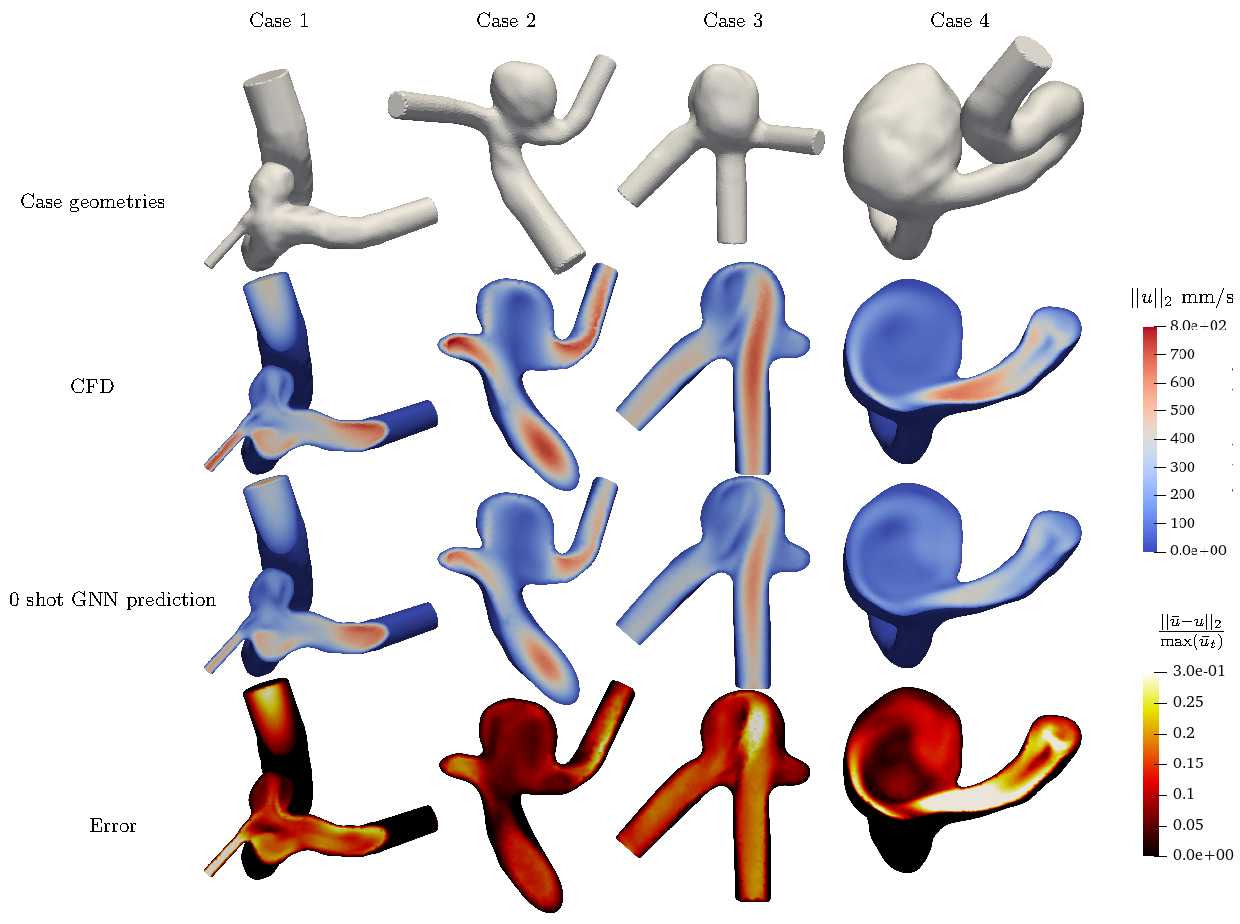
\includegraphics[width=1\textwidth]{figs/0shot_preds.pdf}
\caption{\secondround Zero-shot predictions on out-of-distribution patient-specific ICA and MCA aneurysm cases.}
\label{fig:real_cases}
\end{figure}

\color{black}